\documentclass[conference]{IEEEtran}
\usepackage{cite}
\usepackage{amsmath,amssymb,amsfonts}
\usepackage{algorithmic}
\usepackage{graphicx}
\usepackage{textcomp}
\usepackage{xcolor}
\usepackage{booktabs}
\usepackage{float}

\def\BibTeX{{\rm B\kern-.05em{\sc i\kern-.022em b}\kern-.08em
    T\kern-.1667em\lower.7ex\hbox{E}\kern-.125emX}}

\begin{document}

\title{Visualization Tool for Energy Analysts using CIA Dataset}
\author{
    \IEEEauthorblockN{Harshavardhan Dharman, Surya Kannan, Shashank Venkatesha, Leela Karthikeyan Haribabu}
    \IEEEauthorblockA{\textit{Eindhoven University of Technology}, Eindhoven, Netherlands \\
    \{h.dharman, s.kannan, s.venkatesha, l.k.haribabu\}@student.tue.nl}
}

\maketitle

\begin{abstract}
The Energy Analytics Dashboard is a simple intelligence platform specifically designed to provide energy analysts with a unified environment for cross-sectoral discovery and infrastructure assessment. By integrating five multidisciplinary datasets, the tool enables the analyst to transition seamlessly from geographic overviews to deep multivariate profiling using Coordinated Multiple Views, such as Choropleth Maps, Top-N Rankings, and PCA Cluster plots that reveal hidden peer groups of nations with shared industrial footprints. This design prioritizes "details-on-demand," allowing the user to investigate how physical assets like pipelines and generating capacity drive economic output while highlighting critical structural dependencies essential for policy mapping. The tool’s statistical engine identifies a perfect 1.00 correlation between Total Area and Land Area, alongside exceptionally high correlations between Real GDP and national Imports, confirming the linear scaling of territorial and economic resources. Conversely, it exposes strategic resource trade-offs and land-use tensions for the analyst, most notably a significant low correlation of -0.35 between Agricultural Land and Forest Land. By exposing these high and low correlation values through interactive Parallel Coordinates and heatmaps, the platform empowers the energy analyst to pinpoint "efficiency frontiers" where nations optimize resource allocation. Ultimately, this visualization environment exposes complex industrial interdependencies that traditional, static statistical models often obscure, providing the analyst with a dynamic tool for evidence-based decision-making.
\end{abstract}

\begin{IEEEkeywords}
Energy Analytics, Information Visualization, Multivariate Profiling, Infrastructure Assessment, PCA Clustering.
\end{IEEEkeywords}

\section{Introduction}
\subsection{Motivation and Domain Problem}
In an era of unparalleled global interconnection, there is a challenge in understanding the complex relationships between energy production, economic development, infrastructure, and environmental sustainability across all countries. Traditional statistical tables and reports fail to reveal the nuanced patterns, regional clusters, and multi-dimensional correlations that drive the interdependent link between energy usage and economic growth. The primary domain goal for the energy analyst is to understand how physical energy infrastructure, such as generating capacity and pipelines, correlates with economic health, and to identify patterns such as "high GDP but high carbon intensity" or "expanding infrastructure combined with low energy equity." Current approaches like spreadsheets and static reports make it hard to see these patterns; interactive visualization is well-suited because it leverages spatial position, color, and length as highly effective perceptual channels for comparison and pattern finding.

\subsection{Target Users and Goals}
\textbf{Target User:} The primary user of this tool is the Energy Analyst tasked with synthesizing complex, multi-sector data to guide infrastructure planning and policy decisions.

\textbf{Project Goals:} The primary goal is to facilitate Exploration and Analysis by allowing the analyst to investigate how energy mixes and transport networks support population growth while driving national economic health. Through interactive features like PCA clustering, the tool enables the user to identify "peer nations" with similar industrial footprints. Ultimately, the dashboard allows the analyst to pinpoint "connectivity gaps" and discover "positive deviants" who successfully decouple economic growth from high environmental impact.

\subsection{Why Visualization?}
Visualization is the superior choice because it transforms abstract numbers into actionable spatial and relational patterns. While automated statistical methods can provide summaries, they often operate as "black boxes" that hide nuanced outliers. For the Energy Analyst, a visual interface facilitates Human-in-the-loop Discovery, allowing the user to spot geographic trends through Choropleth Maps. Furthermore, visualization excels at Multivariate Profiling. By using interactive tools like Parallel Coordinates and PCA Cluster plots, the user can "brush" through data to instantly see how different indicators interact. This empowers the analyst to detect "efficiency frontiers" that static algorithmic outputs simply cannot achieve.

\section{Data Analysis}

\subsection{Domain Data Specification}
The visualization utilizes the CIA World Factbook, a comprehensive dataset containing statistical profiles for over 200 countries at the intersection of infrastructure and macroeconomics. Nations are analyzed through five key dimensions:

\textbf{Energy:} Quantifies resource footprints through electricity access, generating capacity, and fossil fuel metrics (coal, gas, petroleum). $CO_2$ emissions are included to evaluate industrial sustainability.

\textbf{Economy:} Measures financial health and industrial scale using absolute values like Real GDP (PPP) and Trade Volume (Exports/Imports), alongside GDP per Capita for relative prosperity.

\textbf{Demographics:} Uses Total Population as the primary metric to contextualize energy demand and the scale of required infrastructure.

\textbf{Transportation:} Focuses on physical connectivity via gas and oil pipeline mileage (km), reflecting the technological maturity of a nation’s distribution networks.

\textbf{Geography:} Defines the physical context through Total/Land Area and land-use types like Forest and Agricultural Land to assess resource potential and spatial constraints.

In our approach, we have synthesized a multi-domain dataset by merging five distinct categories of country-level indicators: Energy, Economy, Demographics, Transportation, and Geography. Each observation in the final processed dataset represents a sovereign state, identified by its unique ISO-Alpha 3 code. To ensure global coverage and facilitate spatial visualization, we performed a name-matching operation between the CIA World Factbook records and the Gapminder ISO database, resolving nomenclature discrepancies (e.g., mapping "Czechia" to the "Czech Republic" to maintain consistency across historical and modern records).

\subsection{Data Abstraction}
The energy dataset is abstracted according to Munzner's data model framework, as shown in Table~\ref{tab:data_abstraction}.

\begin{table}[H]
\centering
\caption{Energy Dataset Abstraction}
\label{tab:data_abstraction}
\small
\begin{tabular}{|p{3.5cm}|p{1.4cm}|p{0.8cm}|p{1.4cm}|}
\hline
\textbf{Attribute} & \textbf{Semantic Type} & \textbf{Data Type} & \textbf{Range} \\
\hline
Country & Categorical & Key (Item) & 260 unique \\
electricity\_access\_percent & Quantitative & Ratio & 0--100\% \\
elec\_generating\_capacity\_kW & Quantitative & Ratio & 0--2.38B \\
coal\_metric\_tons & Quantitative & Ratio & 0--3.69B \\
petroleum\_bbl\_per\_day & Quantitative & Ratio & 0--18.6M \\
refined\_petrol\_products & Quantitative & Ratio & 0--20.3M \\
refined\_petrol\_exports & Quantitative & Ratio & 0--5.92M \\
refined\_petrol\_imports & Quantitative & Ratio & 0--2.19M \\
natural\_gas\_cubic\_m & Quantitative & Ratio & 0--967B \\
carbon\_dioxide\_emissions & Quantitative & Ratio & 0--11.5B Mt \\
iso\_alpha (derived) & Categorical & Key & 200+ unique \\
continent (derived) & Categorical & Ordered & 6 categories \\
\hline
\end{tabular}
\end{table}

\begin{table}[H]
\centering
\caption{Economy Dataset Abstraction}
\small
\begin{tabular}{|l|l|l|l|}
\hline
\textbf{Attribute} & \textbf{Semantic Type} & \textbf{Data Type} & \textbf{Range} \\
\hline
Real GDP (PPP) & Quantitative & Ratio & 0--23,320 \\
GDP per Capita & Quantitative & Ratio & 0--115,700 \\
Exports (B USD) & Quantitative & Ratio & 0--3,527 \\
Imports (B USD) & Quantitative & Ratio & 0--3,401 \\
\hline
\end{tabular}
\end{table}

\begin{table}[H]
\centering
\caption{Demographics Dataset Abstraction}
\small
\begin{tabular}{|l|l|l|l|}
\hline
\textbf{Attribute} & \textbf{Semantic Type} & \textbf{Data Type} & \textbf{Range} \\
\hline
Total Population & Quantitative & Absolute & 0--1.42B \\
\hline
\end{tabular}
\end{table}

\begin{table}[H]
\centering
\caption{Energy Production Summary}
\small
\begin{tabular}{|l|l|l|}
\hline
Source & Type & Global Share \\
\hline
Coal & Fossil & High \\
Oil & Fossil & Medium \\
Renewables & Clean & Growing \\
\hline
\end{tabular}
\end{table}

\begin{table}[H]
\centering
\caption{Task Abstraction Mapping}
\small
\begin{tabular}{|l|l|l|}
\hline
Task & Action & Visualization \\
\hline
Emission Analysis & Discover & Choropleth Map \\
Market Control & Compare & Bar Chart \\
Pattern Detection & Analyze & Scatter Plot \\
\hline
\end{tabular}
\end{table}

\section{Task Analysis}
\subsection{Domain-Specific Tasks}
\textbf{Task 1: Analyze Environmental Impact and Global Emissions}
\begin{itemize}
    \item \textbf{Description}: Identifying drivers of greenhouse gas emissions by analyzing $CO_{2}$ output in relation to industrial scale (see Figure~\ref{fig:large_analysis_view}).
    \item \textbf{Why it matters}: Monitoring carbon footprints is essential for assessing global climate policy and identifying heavy polluters.
    \item \textbf{Questions}: Who are the leading global carbon emitters? Which countries contribute most to global $CO_{2}$ emissions? Is there a correlation between electricity capacity and carbon output?
\end{itemize}

% LARGE IMAGE SPANNING BOTH COLUMNS AT TOP OF NEW PAGE
\clearpage
\begin{figure*}[t]
    \centering
    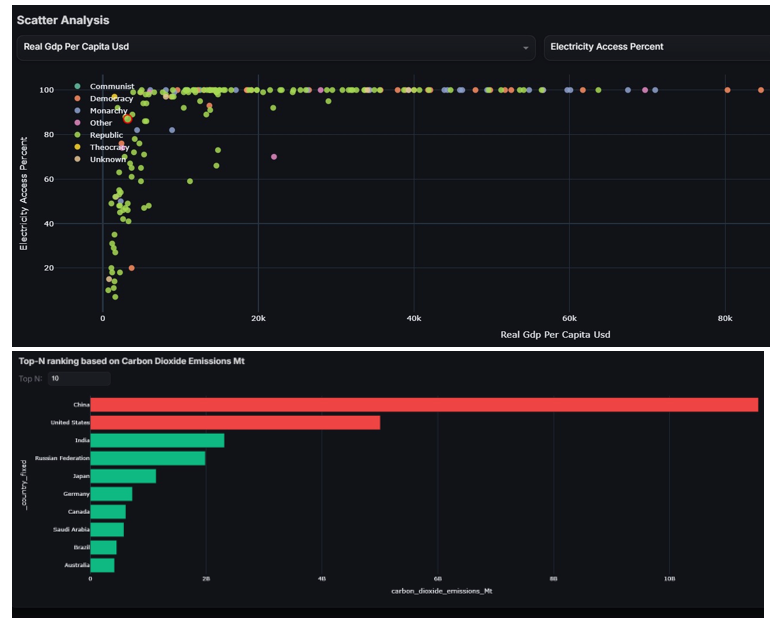
\includegraphics[width=0.95\textwidth]{fig1.png} 
    \caption{Comprehensive Environmental Impact Analysis: Global $CO_{2}$ Emissions vs. Industrial Scale.}
    \label{fig:large_analysis_view}
\end{figure*}

\textbf{Task 2: Correlate Economic Wealth and Energy Access}
\begin{itemize}
    \item \textbf{Description}: Investigating if wealth alone is a sufficient driver for infrastructure (see Figure~\ref{fig:gdp_emission_plot}).
    \item \textbf{Questions}: Does economic wealth guarantee energy access? Is there a strong correlation between $GDP$ per capita and electricity access?
    \item \textbf{Insight}: Moderate correlation (0.46). Higher GDP helps, but policy and geography are equally critical.
\end{itemize}

\begin{figure}[H]
    \centering
    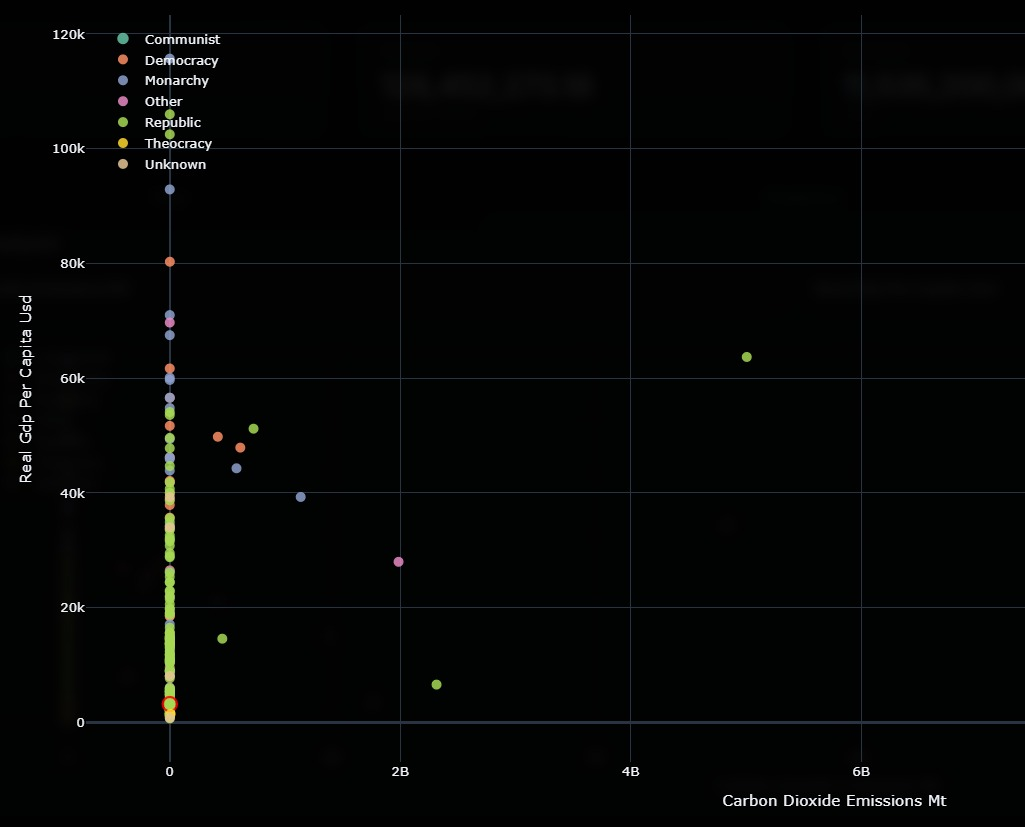
\includegraphics[width=0.8\linewidth]{fig5.jpeg}
    \caption{Real GDP vs Carbon Emission}
    \label{fig:gdp_emission_plot}
\end{figure}

\textbf{Task 3: Analyze Carbon Intensity and Economic Efficiency}
\begin{itemize}
    \item \textbf{Description}: Evaluating efficiency by calculating $CO_{2}$ emissions relative to GDP.
    \item \textbf{Questions}: Which economies are the most "Carbon Intensive"? Who emits the most relative to economic output?
    \item \textbf{Insight}: China and Russia lead major economies. Small island nations show high ratios due to fossil fuel import reliance.
\end{itemize}

\subsection{Task Abstraction}
Mapping domain tasks to generic action-target pairs.

\begin{table}[H]
\centering
\caption{Task Abstraction: Mapping Domain Tasks to Abstract Actions}
\label{tab:task_abstraction}
\small
\begin{tabular}{|p{1.8cm}|p{1.8cm}|p{1.5cm}|p{2.0cm}|}
\hline
\textbf{Domain Task} & \textbf{Action} & \textbf{Target} & \textbf{Idiom Support} \\
\hline
Discover spatial patterns & Discover & Distribution & Choropleth Map \\
\hline
Generate hypotheses & Discover & Dependency & Scatter Plot \\
\hline
Characterize profiles & Derive & Clusters & PCA + K-Means \\
\hline
Correlate attributes & Identify & Correlation & Scatter Plot, Corr. Matrix \\
\hline
Identify extremes & Identify & Extremes & Bar Chart (Top-N) \\
\hline
Filter by region & Filter & Items & Continent Dropdown \\
\hline
Lookup value & Lookup & Value & Hover Tooltip \\
\hline
Locate country & Locate & Position & Geographic Map \\
\hline
Select \& highlight & Select & Item & Click interaction \\
\hline
Brush range & Filter & Range & Parallel Coordinates \\
\hline
\end{tabular}
\end{table}

\begin{table}[H]
\centering
\caption{Idiom Justification and Theoretical Mapping}
\label{tab:idiom_justification}
\small
\begin{tabular}{|p{2.2cm}|p{5.5cm}|}
\hline
\textbf{Idiom} & \textbf{Justification (Why we use it)} \\
\hline
Choropleth Map & Encodes data into spatial regions via color to reveal geographic distributions. \\
\hline
Scatter Plot & Best for identifying dependencies/trends using high-precision position channels. \\
\hline
PCA + K-Means & Derives and visualizes hidden clusters within multi-dimensional datasets. \\
\hline
Bar Chart & Uses the length channel for accurate magnitude comparison and ranking. \\
\hline
Corr. Matrix & Provides a high-level summary of all statistical relationships via color saturation. \\
\hline
Parallel Coords & Enables multivariate profiling and range-based filtering via interactive brushing. \\
\hline
\end{tabular}
\end{table}

\section{Visualization Design (HOW)}
\subsection{Visual Channel Selection}
Our visual encodings follow Munzner's effectiveness rankings for quantitative data. Position is the most effective channel and is used in scatter plots for X and Y axes, in the PCA embedding, and in the choropleth map for spatial location. Length is used in bar charts for ranking comparison. Color saturation and hue are used in the choropleth with a Blues scale for sequential data, in the correlation matrix with a diverging RdBu scale, and for continent-based coloring across all scatter-based views.

\subsection{Interaction Design}
Linked views support Shneiderman's Visual Information Seeking Mantra of overview first, zoom and filter, then details-on-demand. The choropleth map provides an overview showing global energy distribution at a glance. Zoom and filter capabilities are provided through the continent dropdown that filters all views and through parallel coordinates brushing that narrows the displayed range. Details-on-demand are available through hover tooltips that reveal exact values and through the comparison table that provides detailed country profiles. View linking is achieved by clicking a country on the map, which highlights it in scatter plots, PCA, and parallel coordinates bidirectionally.

\section{Use Case: Energy Analyst Exploration}
This section demonstrates an extensive data exploration process conducted by an energy analyst using the tool.

\subsection{Scenario}
An energy analyst at a policy research institute seeks to understand the relationship between energy production, carbon emissions, and electricity access across different regions. The goal is to identify countries that could serve as models for sustainable energy development.

\subsection{Exploration Process}
The analyst begins by viewing electricity access percentage on the choropleth map in Step 1, the overview. Immediately visible patterns emerge as Europe and North America show near-universal access represented in deep purple, while Sub-Saharan Africa shows significant gaps shown in yellow. The analyst clicks on several African countries to highlight them for further investigation.

In Step 2, correlation discovery, the analyst switches to the Analytics tab and plots petroleum production in barrels per day on the X-axis against carbon dioxide emissions on the Y-axis. A strong positive correlation is visible. However, the highlighted African countries from Step 1 appear as outliers with low petroleum production but varying emissions. The analyst identifies Nigeria as an exception showing high petroleum production but relatively moderate emissions.

Step 3 involves pattern identification using PCA clustering. The analyst discovers that countries naturally cluster into three groups. The first cluster in blue contains high-emission industrialized nations including the USA, China, and Russia. The second cluster in green contains moderate energy producers with balanced profiles. The third cluster in orange contains low-access developing nations concentrated in Africa.

In Step 4, detailed comparison, the analyst selects Germany, Norway, and Saudi Arabia for comparison representing different energy strategies. The comparison table reveals that Norway has high electricity generating capacity but low carbon emissions due to hydropower, while Saudi Arabia shows high petroleum production and proportionally high emissions.

Finally, Step 5 involves multivariate analysis using parallel coordinates. Brushing to select countries with electricity access above 95 percent and carbon emissions below 100 megatons reveals a subset of nations that achieve high access with low environmental impact including Norway, Sweden, France, and several smaller European nations.

\subsection{Insights Discovered}
Through interactive exploration, the analyst discovered several important findings. First, decoupling energy development from carbon emissions is possible, as several countries achieve near-universal electricity access with low carbon emissions, suggesting that energy development need not be carbon-intensive. Second, regional patterns emerged showing that geographic clustering of energy access gaps aligns with development status but not always with resource availability. Third, trade-offs were identified through the bubble chart, which revealed that natural gas producers often have lower emissions per unit of electricity generation compared to coal producers.

\subsection{Future Work}
Several enhancements would strengthen this visualization tool. A temporal slider incorporating historical data would enable time-series comparison to track how countries' energy profiles evolve. Computing derived attributes such as per-capita and efficiency metrics by merging with demographic data would deepen analytical capabilities. Axis reordering allowing users to drag axes in parallel coordinates for correlation-based ordering would improve the multivariate view. Export functionality enabling analysts to export filtered subsets for external analysis would support integration with other tools. Finally, guided tours providing preset exploration paths for common analytical scenarios would help new users learn the system effectively.

\section{Implementation}
The tool is implemented entirely in Python, using Dash for web-based UI construction and Plotly for interactive visualizations. Data cleaning employs Pandas and regular-expression–based preprocessing. ISO code and continent inference use external libraries such as pycountry, pycountry convert, and gapminder. To achieve Multi View coordination, Dash creates Callbacks that link the state (i.e., clickData, relayoutData, and dcc.Store) of the respective components together. The technical challenges we encountered while developing the system included inconsistent Country names from the CIA database; Missing or Non-numeric; Handling large heterogeneous datasets; Maintaining a uniform display of a stable map; Linking map and scatter selection using ISO-code matching; Designing a Dark-Themed Responsive UI with animated transition, Full-Screen modal, and Vertical Scrollable Containers. The final system integrates all components cohesively while remaining modular for future extension.

\section{Conclusion and Future Work}
\subsection{Summary of Results}
This project developed an interactive visualization tool that enables energy analysts to explore the CIA Energy Dataset across 260 countries. The tool successfully supports a hierarchy of analytical tasks from high-level pattern discovery to low-level value retrieval through coordinated multiple views including choropleth maps, scatter plots, parallel coordinates, PCA clustering, and comparison tables.

\subsection{Benefits and Limitations}
The tool offers several important benefits. Linked views enable seamless exploration from overview to detail, allowing analysts to quickly drill down into specific countries of interest. Multiple visualization idioms support different task types including comparison, correlation analysis, and clustering. Interactive filtering allows hypothesis testing through selection and brushing operations. The dark theme with animations provides a professional and modern user experience.

However, several limitations should be noted. The CIA dataset represents a single point in time, preventing temporal trend analysis that would reveal how energy profiles have changed over years. Approximately 15 percent of country-indicator pairs contain missing values, reducing coverage for some nations. Additionally, the lack of derived metrics such as emissions per capita or emissions per kilowatt-hour limits the depth of analysis.

\subsection{Reflection on Design Choices}
Our initial choice of a choropleth map proved effective for revealing spatial patterns in electricity access, as the geographic encoding immediately communicated regional disparities. However, for attributes without clear geographic patterns such as natural gas production, a sorted bar chart would be more effective.

The parallel coordinates view, while powerful for multivariate filtering, suffers from axis overlap when all nine indicators are displayed. Allowing users to reorder or subset axes would improve usability. The PCA clustering successfully revealed country groupings but lacks interpretability, and adding loading vectors would help analysts understand which attributes drive cluster separation.

\end{document}